\chapter{Versuch 3: Leistungsaufnahme eines Widerstand}

\section{Einleitung}
Das Ziel dieses Versuchs besteht darin, die elektrische Leistung zu bestimmen,
die bei Stromdurchfluss durch einen Widerstand R auftritt. Hierfür werden zwei 
unterschiedliche Methoden verwendet. Zum einen wird die Leistung mittels 
direkter Strommessung bestimmt. Zum anderen wird die elektrische Leistung durch
indirekte Strommessung, d.h. über die Spannungsmessung bestimmt. Anschließend 
sollen die Ergebnisse nach Fehlern untersucht und vergliechen werden.

\section{Benötigte Geräte}
Zur Durchführung des Versuchs werden folgende Geräte und Material benötigt:

\begin{tabular}[h]{c|c}
	Widerstand, zwei Stück & 1 k$\Omega$ \textpm 5\% \\
    \hline
    Digital-Multimeter & Fluke TRUE RNS MULTIMETER\\
    \hline
    Steckbrett & \\
    \hline
    Netzgerät & Tenma 72-10495 Digital Control DC Power Supply
    \label{tab:Versuch 3: Geräte}
\end{tabular}

\section{Durchführung}
\subsection{Ausgemessung der Widerstände}
Um die Genauigkeit zu erhöhen, werden die zwei Widerstände R\textsubscript{1}
und R\textsubscript{2} ausgemessen. Widerstand R\textsubscript{1} hat den 
Wert 0,996 k$\Omega$ und Widerstand R\textsubscript{2} hat den Wert 0,996 
k$\Omega$. Somit liegen die Widerstände innerhalb des von dem Hersteller
angegebenen Toleranzbereiches \textpm 5\%. 

\subsection{Direkte Strommessung}
Es wird eine Schaltung aufgebaut, um die Leistung zu bestimmen. Dafür werden
Netzgerät, Widerstand R\textsubscript{1} und Strommessgerät (DMM) in Reihe
geschaltet. Schaltskizze sieht folgendermaßen aus:

\begin{figure}[H]
	\centering
	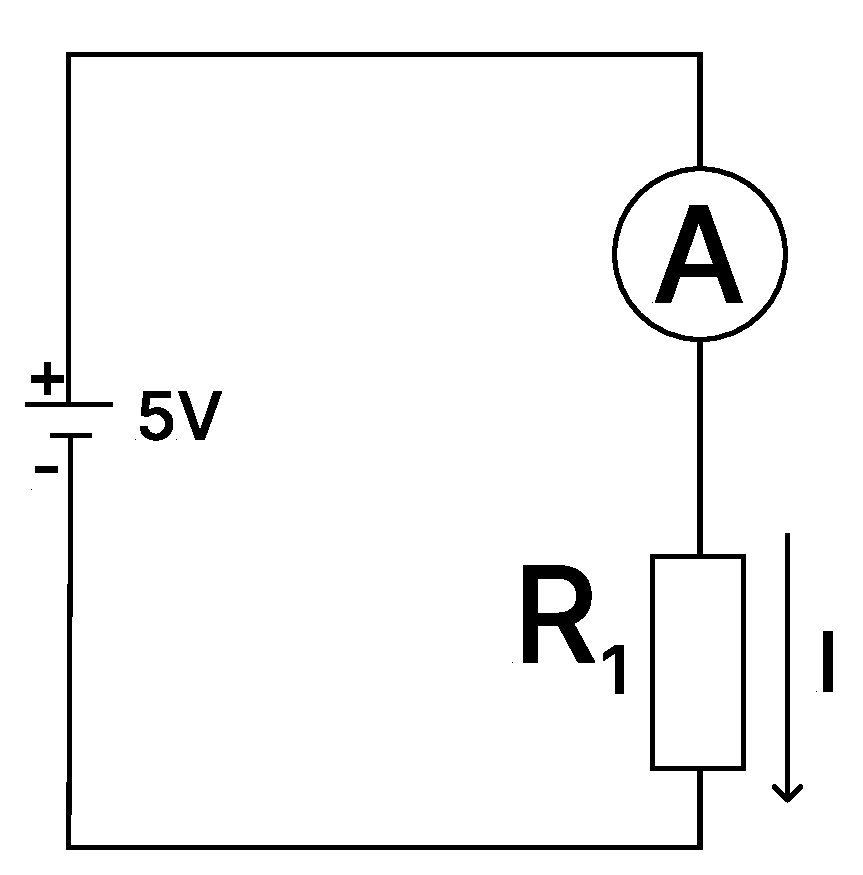
\includegraphics[height=6cm]{images/Versuch3/Versuch3_1_Schaltskizze.pdf} 
	\caption{Schaltungsskizze}
	\label{fig: Schaltungsskizze Versuch 3}
\end{figure}

Mit Hilfe des DMMs wird der Strom gemessen. Dieser beträgt 5.01 mA. Mit der
Formel $P = I^{2}R$ wird die Leistung bestimmt: $P=(5,01 mA)^{2}\cdot 0,996 k\Omega = 0,0249 W$.
XXXFEHLERRECHNUNGXXX

\subsection{Indirekte Strommessung}
Jetzt soll die elektrische Leistung mit der Methode der indirekten Strommessung
bestimmt werden. Dafür werden der zweite Widerstand, sowie der Spannungsmessgerät
(DMM) in die Schaltung eingebaut. Als R\textsubscript{V} dient der
zweite Widerstand. Die Schaltskizze sieht folgendermaßen aus:

\begin{figure}[H]
	\centering
	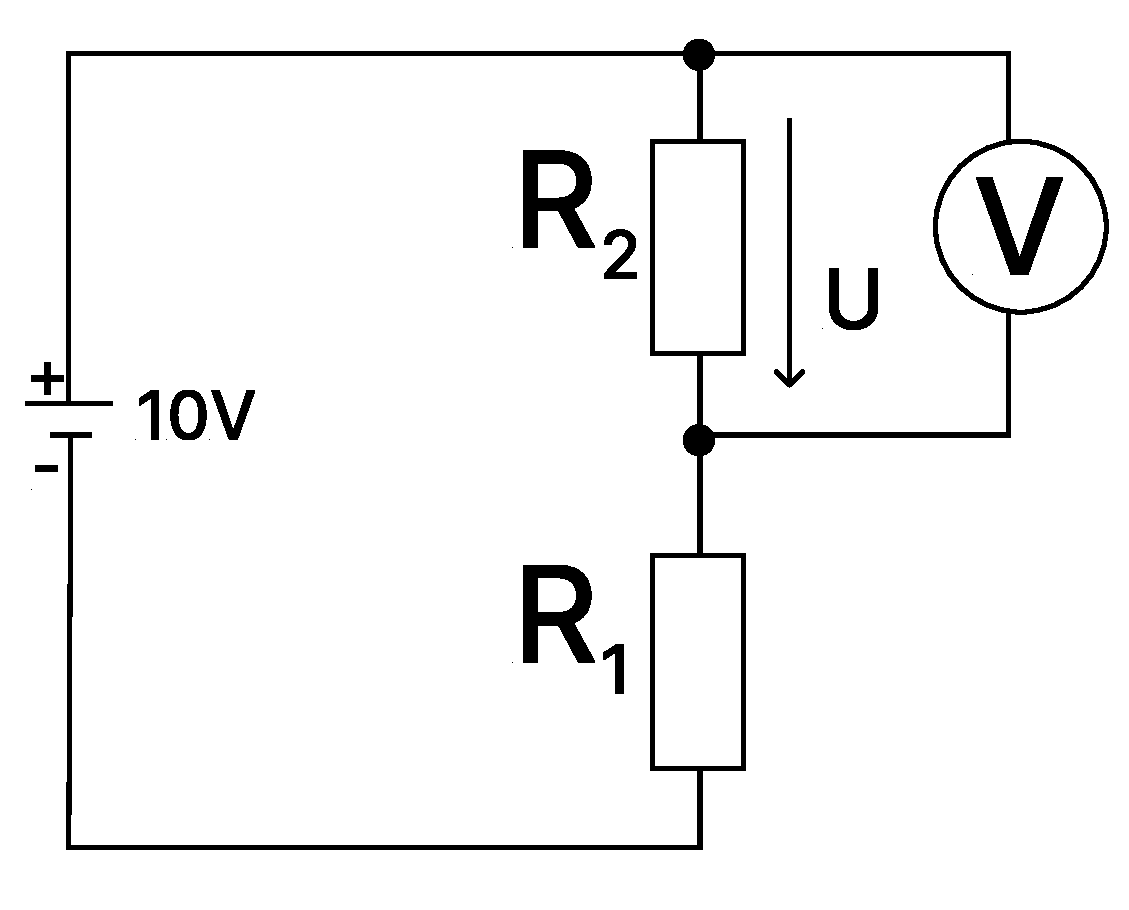
\includegraphics[height=6cm]{images/Versuch3/Versuch3_2_Schaltskizze.pdf} 
	\caption{Schaltungsskizze}
	\label{fig: Schaltungsskizze Versuch 3_2}
\end{figure}

Mit Hilfe des DMMs wird die Spannung gemessen. Diese beträgt 4,964 V. Mit der
Formel $P = (\frac{U}{R\textsubscript{V}})^{2}R$ wird die Leistung bestimmt: 
$P = (\frac{4,954 V}{0,985 k\Omega})^{2}\cdot 0,996k\Omega = 0,0252 W$.

XXXFEHLERRECHNUNGXXX